\documentclass[a4paper,table]{report}
\input{preamble.tex}
\input{definitions2.tex}
\input{tikz.tex}
\input{myboxes.tex}

\usepackage[cmtip,all]{xy}
\usepackage{silence}
\WarningsOff[catoptions]
\usepackage{extarrows}

\geometry{left=9mm,right=9mm,top=30.00mm,bottom=34.00mm,footskip=24.16mm,headsep=24.16mm}
\everymath{\displaystyle}
\pagestyle{vangelis}



\begin{document}

\chapter{Παράγωγος Κατά Κατεύθυνση}

\section{Ανάδελτα - Κλίση - Λαπλασιανή}

\begin{dfn}[Τελεστής Hamilton ή Ανάδελτα]
  \[ \grad = \pdv{}{x} \mathbf{i} + \pdv{}{y} \mathbf{j} + \pdv{}{z} \mathbf{k} \quad
  \text{ή} \quad \grad = \left(\pdv{}{x} , \pdv{}{y} , \pdv{}{z}\right)  \]
\end{dfn}

\begin{dfn}
  Έστω $ f(x,y,z) $ συνάρτηση. Τότε η διανυσματική συνάρτηση 
  \[ \grad f = \pdv{f}{x} \mathbf{i}+ \pdv{f}{y} \mathbf{j} + \pdv{f}{z} \mathbf{k} 
  \quad \text{ή} \quad \grad f = \left(\pdv{f}{x} , \pdv{f}{y} , \pdv{f}{z}\right)\]
  ονομάζεται \textcolor{Col1}{κλίση} της συνάρτησης $ f(x,y,z) $.
\end{dfn}

\begin{dfn}[Τελεστής Laplace]
  \[ 
    \Delta \overset{\text{ή}}{=} \laplacian = \pdv[2]{}{x} + \pdv[2]{}{y} 
    \quad \text{ή} \quad 
    \Delta \overset{\text{ή}}{=} \laplacian = \pdv[2]{}{x} + \pdv[2]{}{y} + \pdv[2]{}{z} 
  \]
\end{dfn}

\begin{dfn}
  Έστω $ f(x,y,z) $ συνάρτηση. Τότε η πραγματική συνάρτηση 
  \[ 
    \Delta f \overset{\text{ή}}{=} \laplacian f = \pdv[2]{f}{x} + \pdv[2]{f}{y} + \pdv[2]{f}{z} 
  \]
  ονομάζεται \textcolor{Col1}{Λαπλασιανή} της συνάρτησης $ f(x,y,z) $.
\end{dfn}


\section{Αρμονικές Συναρτήσεις - Εξίσωση Laplace}

\begin{dfn}
  Η συνάρτηση $ f(x,y) $ λέγεται \textcolor{Col1}{αρμονική} αν ικανοποιεί την
  εξίσωση $ \Delta f = 0 $ ή ισοδύναμα $ \laplacian f = 0 $.  Δηλαδή 
  \[
    \pdv[2]{f}{x} + \pdv[2]{f}{y} = 0  
  \]
\end{dfn}

\begin{rem}
  \item {}
    \begin{enumerate}
      \item Η παραπάνω εξίσωση, ονομάζεται \textcolor{Col1}{εξίσωση Laplace}.
      \item Η εξίσωση Laplace για συναρτήσεις πολλών μεταβλητών παίρνει τη 
        μορφή
        \[
          \pdv[2]{f}{x_{1}} + \pdv[2]{f}{x_{2}} + \cdots + 
          \pdv[2]{f}{x_{n}}=0 
        \] 
    \end{enumerate}
  \end{rem}

  \begin{prop}
  \item {}
    Αν $ f(x,y) $ συνεχής, έχει συνεχείς μερικές παραγώγους 1ης τάξης 
    και είναι αρμονική, τότε και οι συναρτήσεις $ f_{x} $ και $ f_{y} $
    είναι αρμονικές. 
  \end{prop}

  \begin{proof}
  \item {}
    $f$ αρμονική $ \Rightarrow f_{xx}+f_{yy}=0 $.

    Θέτουμε $ g(x,y)=f_{x}(x,y) $. Για να δείξουμε ότι $ f_{x} $ αρμονική, 
    αρκεί να δείξουμε ότι $ g(x,y) $ είναι αρμονική. Πράγματι:
    \begin{align*}
      g_{x} &= f_{xx} \quad \text{και} \quad g_{xx} = (f_{xx})_{x} \\ 
      g_{y} &= f_{xy} \quad \text{και} \quad g_{yy} = (f_{xy})_{y} =
      (f_{yx})_{y} = f_{yxy} = f_{yyx} = (f_{yy})_{x}
    \end{align*}
    Άρα 
    \[
      g_{xx}+g_{yy} = (f_{xx})_{x} + (f_{yy})_{x} = 
      (f_{xx}+f_{yy})_{x}= (0)_{x} =0
    \] 
  \end{proof}

  \begin{example}
    Να εξεταστεί αν η συνάρτηση $ f(x,y)= \ln{\sqrt{x^{2}+y^{2}}} $ είναι αρμονική.
  \end{example}
  \begin{solution}
    \begin{align*}
      \pdv{f}{x} &= f_{x} = \left(\ln{\sqrt{x^{2}+y^{2}}} \right)_{x} = 
      \frac{1}{\sqrt{x^{2}+y^{2}}} \cdot 
      \left(\sqrt{x^{2}+y^{2}}\right)_{x} = 
      \frac{1}{\sqrt{x^{2}+y^{2}}} \cdot \frac{\cancel{2}x}{\cancel{2} 
      \sqrt{x^{2}+y^{2}}} = \frac{x}{x^{2}+y^{2}} \\
      \pdv[2]{f}{x} &= f_{xx} = \left(\frac{x}{x^{2}+y^{2}}\right)_{x} = 
      \frac{x^{2}+y^{2}-2x^{2}}{(x^{2}+y^{2})^{2}} = 
      \frac{y^{2}-x^{2}}{(x^{2}+y^{2})^{2}} 
      \intertext{και}
      \pdv{f}{y} &= f_{y} = \left(\ln{\sqrt{x^{2}+y^{2}}} \right)_{y} = 
      \frac{1}{\sqrt{x^{2}+y^{2}}} \cdot 
      \left(\sqrt{x^{2}+y^{2}}\right)_{y} = 
      \frac{1}{\sqrt{x^{2}+y^{2}}} \cdot \frac{\cancel{2}y}{\cancel{2} 
      \sqrt{x^{2}+y^{2}}} = \frac{y}{x^{2}+y^{2}} \\
      \pdv[2]{f}{y} &= f_{yy} = \left(\frac{y}{x^{2}+y^{2}}\right)_{y} = 
      \frac{x^{2}+y^{2}-2y^{2}}{(x^{2}+y^{2})^{2}} = 
      \frac{x^{2}-y^{2}}{(x^{2}+y^{2})^{2}} 
    \end{align*}  
    Προφανώς έχουμε ότι
    \[
      \pdv[2]{f}{x} + \pdv[2]{f}{y} = f_{xx}+f_{yy} =
      \frac{y^{2}-x^{2}}{(x^{2}+y^{2})^{2}} + 
      \frac{x^{2}-y^{2}}{(x^{2}+y^{2})^{2}} = 0  
    \] 
  \end{solution}

  \section{Παράγωγος κατά Κατεύθυνση}

  \begin{dfn}
    Η \textcolor{Col1}{παράγωγος κατά κατεύθυνση} της \textbf{διαφορίσιμης} συνάρτησης 
    $ f(x,y) $ στο σημείο $ P(x_{0}, y_{0}) $ και προς την κατεύθυνση του διανύσματος 
    $ \mathbf{u} $ δίνεται από τον τύπο
    \[
      \dv{f}{s} \overset{\text{ή}}{=} \dv{f}{\mathbf{u}} 
      \overset{\text{ή}}{=} D_{\mathbf{u}}(f)(P) = \grad f(P) \cdot \mathbf{\widehat{u}} 
    \] 
    όπου $ \grad f (P) $ είναι η κλίση της συνάρτησης $f$ στο σημείο $P$ και 
    $ \mathbf{\widehat{u}} $ είναι το \textbf{μοναδιαίο} διάνυσμα $ \mathbf{u} $.
  \end{dfn}
  \begin{example}
    Έστω η συνάρτηση $ f(x,y) = 100-x^{2}-y^{2} $. 
    \begin{enumerate}[i)]
      \item Να βρείτε την παράγωγο της $f$ στο σημείο $ P_{0}(3,4) $ και προς την 
        κατεύθυνση του \textbf{διανύσματος} $ \mathbf{u} = 3 \mathbf{i}- 4 \mathbf{j} $.
      \item Να βρείτε την παράγωγο της $f$ στο σημείο $ P_{0}(3,4) $ και προς την 
        κατεύθυνση του \textbf{σημείου} $P(1,2)$.
      \item Προς ποια κατεύθυνση η $f$ αυξάνει με το \textbf{μεγαλύτερο ρυθμό}, 
        στο σημείο $ P_{0} $; Ποιος είναι ο μέγιστος ρυθμός μεταβολής της $f$;
      \item Προς ποια κατεύθυνση η παράγωγος κατά κατεύθυνση γίνεται \textbf{μηδέν}; στο 
        σημείο $ P_{0} $;
    \end{enumerate}
  \end{example}
  \begin{solution}
    \begin{enumerate}[i)]
      \item Έχουμε ότι $ D_{\mathbf{u}}f(P_{0}) = \grad f(P_{0}) \cdot 
        \mathbf{\widehat{u}} $
        \begin{align*}
          \grad f = (f_{x}, f_{y}) = (-2x, -2y) \Rightarrow \grad f(P_{0}) = (-6,-8) \\
          \mathbf{\widehat{u}} = \frac{\mathbf{u}}{\norm{\mathbf{u}}} =
          \frac{1}{\sqrt{3^{2}+(-4)^{2}}} (3,-4) = \left(\frac{3}{5} , - 
          \frac{4}{5}\right)
        \end{align*} 
        Επομένως
        \[
          D_{\mathbf{u}}f(P_{0}) = (-6,-8) \cdot \left(\frac{3}{5} , - \frac{4}{5}\right) 
          = - \frac{18}{5} + \frac{32}{5} = \frac{14}{5} > 0
        \] 
      \item Βρίσκουμε το διάνυσμα $ \vec{P_{0}P} = (1-3,2-4) = (-2,-2) $. Τότε το 
        μοναδιαίο $ \vec{\widehat{P_{0}P}} =
        \frac{\vec{P_{0}P}}{\norm{\vec{P_{0}P}}} = \frac{1}{\sqrt{8}} (-2,-2) = \left(-
        \frac{1}{\sqrt{2}} , - \frac{1}{\sqrt{2}}\right) $
        Άρα 
        \[
          D_{\mathbf{P_{0}P}}f(P_{0}) = \grad f(P_{0}) \cdot \vec{P_{0}P} = (-6,-8) 
          \cdot \left(- \frac{1}{\sqrt{2}} , - \frac{1}{\sqrt{2}}\right) = 
          \frac{6}{\sqrt{2}} + \frac{8}{\sqrt{2}} = \frac{14}{\sqrt{2}} > 0
        \] 
      \item Ζητάμε την κατεύθυνση $ \mathbf{u} $ προς την οποία η $f$ αυξάνει με το 
        μεγαλύτερο ρυθμό, δηλαδή η παράγωγος κατά κατεύθυνση γίνεται μέγιστη. Έχουμε:
        \[
          D_{\mathbf{u}}f(P_{0}) \max \Leftrightarrow \norm{\grad f (P_{0})}
          \norm{\mathbf{\widehat{u}}} \cos{\theta} \max \Leftrightarrow 
          \norm{\grad f(P_{0})} \cos{\theta} \max \Leftrightarrow \cos{\theta} \max
          \Leftrightarrow \theta = 0
        \]
        Δηλαδή $ \mathbf{u} $ παράλληλο με $ \grad f(P_{0}) $. Οπότε, η $f$ αυξάνει με 
        το μεγαλύτερο ρυθμό, προς την κατεύθυνση της κλίσης της. Μάλιστα, ισχύει:
        \[
          - \norm{\grad f(P_{0})} \leq D_{\mathbf{u}} f(P_{0}) \leq \norm{\grad f(P_{0})}
        \]
        για κάθε κατεύθυνση $ \mathbf{u} $ στο σημείο $ P_{0} $. 
        Δηλαδή, ο \textbf{μέγιστος ρυθμός} μεταβολής της $f$ στο σημείο $ P_{0} $ είναι $
        D_{\mathbf{u}}f(P_{0})_{\max} = \norm{\grad f(P_{0})} $ και παρατηρείται προς 
        την κατεύθυνση που δείχνει η κλίση, και ο \textbf{ελάχιστος ρυθμός} μεταβολής
        αντίστοιχα, είναι $ D_{\mathbf{u}}f(P_{0})_{\min} = -\norm{\grad f(P_{0})} $ 
        και παρατηρείται προς την αντίθετη κατεύθυνση από αυτή της κλίσης.
      \item Έχουμε ότι 
        \[ 
          D_{\mathbf{u}}f(P_{0}) = 0 \Leftrightarrow \norm{\grad f (P_{0})}
          \norm{\mathbf{\widehat{u}}} \cos{\theta} = 0 \Leftrightarrow 
          \cos{\theta} = 0 \Leftrightarrow \theta = \pi/2 
        \]
        Δηλαδή, προς κατεύθυνση \textbf{κάθετη} προς την κατεύθυνση που μας δείχνει η 
        κλίση της $ f $ στο σημείο $ P_{0} $, ο ρυθμός μεταβολής της συνάρτησης είναι 
        μηδέν, και επομένως η $f$ είναι σταθερή. Για να προσδιορίσουμε το διάνυσμα $
        \mathbf{u} $, έχουμε: Έστω $ \mathbf{u} = (u_{1}, u_{2}) $. 
        \[
          \mathbf{u} \perp \grad f(P_{0}) \Leftrightarrow \mathbf{u} \cdot 
          \grad f (P_{0}) = 0 \Leftrightarrow (u_1,u_{2}) \cdot (-6,-8) =
          0 \Leftrightarrow \inlineequation[eq:perp]{-6u_{1}-8u_{2}=0}
        \]
        Επίσης, επειδή $ \mathbf{u} $ είναι μοναδιαίο, έχουμε: 
        \[
          \norm{\mathbf{u}} =1 \Leftrightarrow \sqrt{u_{1}^{2}+u_{2}^{2}} = 1
          \Leftrightarrow \inlineequation[eq:unit]{u_{1}^{2}+u_{2}^{2}=1}
        \] 
        Από τις παραπάνω σχέσεις, για τα $ u_{1} $ και $ u_{2} $, εύκολα τα υπολογίζουμε,
        και βρίσκουμε ότι $ \mathbf{u} = \left(- \frac{4}{5}
        , \frac{3}{5}\right) $ ή $ \mathbf{u} = 
        \left( \frac{4}{5} , - \frac{3}{5}\right) $. 
    \end{enumerate}
  \end{solution}

  \section{Σχέση Διαφορικού με Παράγωγο κατά Κατεύθυνση}

  Το διαφορικό μιας συνάρτησης μπορεί να πάρει τη μορφή 
  \[
    df = (\grad f(P_{0})\cdot \hat{\mathbf{u}}) ds = \grad f(P_{0})\cdot d \mathbf{r} 
  \] 
  Οπότε αν λάβουμε υπόψη μας ότι $ d \mathbf{r} = dx \mathbf{i}+ dy \mathbf{j}+ dz
  \mathbf{k} $ και κάνουμε την πράξη του εσωτερικού γινομένου, προκύπτει ο γνωστός τύπος
  \[
    df = f_{x}dx + f_{y}dy+ f_{z}dz 
  \]
  \begin{rem}
    Η Γεωμετρική ερμηνεία των παραπάνω τύπων είναι:
    \begin{myitemize}
      \item Το $ (\grad f({_{0}})\cdot \hat{\mathbf{u}})ds $ μας δίνει τη μεταβολή της 
        $f$ αν μετακινηθούμε από το $ P_{0} $ κατά ds προς την κατεύθυνση του
        διανύσματος $ \hat{\mathbf{u}} $.
      \item Το $ \grad f({_{0}})\cdot \mathbf{r} $ μας δίνει τη μεταβολή της 
        $f$ αν μετακινηθούμε από το $ P_{0} $ κατά $ d \mathbf{r} $. 
    \end{myitemize}
  \end{rem}
  \begin{example}
    Να υπολογιστεί η μεταβολή του βαθμωτού πεδίου $ f(x,y,z)= y \sin{x} +2yz $ αν το 
    σημείο $ P(x,y,z) $ μετακινηθεί από $ P_{0}(0,1,0) $ προς το $ P_{1}(2,2,-2) $ πάνω 
    σε ευθεία διανύοντας απόσταση $ \Delta s = 0.1 $ μονάδες.
  \end{example}
  \begin{solution}
  \item {}
    \begin{myitemize}
      \item $ \grad f = (y \cos{x} , \sin{x} +2z, 2y) $
      \item $ \grad f(P_{0}) = (1,0,2) $
      \item $ \mathbf{u} = \mathbf{P_{0}P_{1}} = (2-0,2-1,-2-0) = (2,1,-2) $
      \item $ \hat{\mathbf{u}} = \frac{\mathbf{P_{0}P_{1}}}{\norm{\mathbf{P_{0}P_{1}}}} =
        \frac{1}{\sqrt{9}} (2,1,-2) = \frac{1}{3} (2,1,-2) $
    \end{myitemize}
    Άρα $ df = (\grad f(P_{0})\cdot \hat{\mathbf{u}}) ds = \left[(1,0,2) \cdot
    \frac{1}{3} (2,1,-2)\right]\cdot 0.1 = - \frac{2}{3}\cdot 0,1 $.
  \end{solution}



  \chapter{Παράγωγος Σύνθετων Συναρτήσεων}

  \section{1η Περίπτωση: \ensuremath{z=f(x,y),  x=x(t),  y=y(t)}} 

  \begin{thm}
    Αν η συνάρτηση $ f(x,y) $ είναι ορισμένη στο ανοιχτό σύνολο 
    $ A \subseteq \mathbb{R}^{2} $ και $ x = x(t) $, $ y=y(t) $, με 
    $ t \in [a,b] $ και η $f$ έχει συνεχείς μερικές 
    παραγώγους στο $A$ και οι $ x(t) $ και $ y(t) $ είναι παραγωγίσιμες στο 
    $ [a,b] $, τότε η παράγωγος της σύνθετης συνάρτησης $f$ ως προς $t$ δίνεται από 
    τον τύπο:

    \vspace{\baselineskip}

    \twocolumnsideslc{
      \begin{center}
        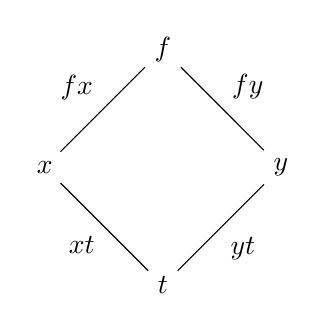
\begin{tikzpicture}
          \node (f) at (0,0) {$f$};  
          \node (x) at (-1.5,-1.5) {$x$};  
          \node (y) at (1.5,-1.5) {$y$};  
          \node (t) at (0,-3) {$t$};  
          \draw (f) edge node[midway,above left] {$\pdv{f}{x}$} (x) ;
          \draw (f) edge node[midway,above right] {$\pdv{f}{y}$} (y) ;
          \draw (x) edge node[midway,below left] {$\dv{x}{t}$} (t) ;
          \draw (y) edge node[midway,below right] {$\dv{y}{t}$} (t) ;
        \end{tikzpicture}
      \end{center}
    }{
      \begin{equation}\label{eq:deriv1}
        \dv{f}{t} = \pdv{f}{x} \dv{x}{t} + \pdv{f}{y} \dv{y}{t} 
      \end{equation}
      Ενώ η 2η παράγωγος από τον τύπο:
      \[
        \dv[2]{f}{t} =  \pdv[2]{f}{x} \left(\dv{x}{t}\right)^{2} + 
        2 \pdv[2]{f}{x}{y} \dv{x}{t} \dv{y}{t} + \pdv[2]{f}{y} 
        \left(\dv{y}{t}\right)^{2} + \pdv{f}{x} \dv[2]{x}{t} + \pdv{f}{y} \dv[2]{y}{t}
      \]
    }
  \end{thm}

  \section{2η Περίπτωση: \ensuremath{z=f(x,y),  x=x(u,v),  y=y(u,v)}} 

  \begin{thm}
    Αν η συνάρτηση $ f(x,y) $ είναι ορισμένη στο ανοιχτό σύνολο 
    $ A \subseteq \mathbb{R}^{2} $ και $ x = x(u,v) $, $ y=y(u,v) $, με 
    και η $f$ έχει συνεχείς μερικές παραγώγους στο $A$ και οι $ x $ και $ y $, έχουν 
    συνεχείς μερικές παραγώγους στο $ E \subseteq \mathbb{R}^{2} $,
    τότε οι μερικές παράγωγοι της $f$, υπάρχουν και δίνονται από τους τύπους:
  \end{thm}

  \twocolumnsideslc{ 
    \begin{center}
      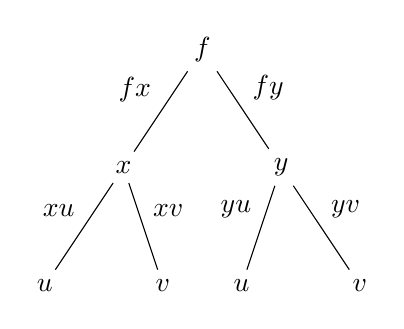
\begin{tikzpicture}
        \node (f) at (0,0) {$f$};  
        \node (x) at (-1,-1.5) {$x$};  
        \node (y) at (1,-1.5) {$y$};  
        \node (ux) at (-2,-3) {$u$};  
        \node (vx) at (-0.5,-3) {$v$};  
        \node (uy) at (0.5,-3) {$u$};  
        \node (vy) at (2,-3) {$v$};  
        \draw (f) edge node[midway,above left] {$ \pdv{f}{x}$} (x) ;
        \draw (f) edge node[midway,above right] {$ \pdv{f}{y}$} (y) ;
        \draw (x) edge node[midway,above left] {$ \pdv{x}{u}$} (ux) ;
        \draw (x) edge node[midway,above right] {$ \pdv{x}{v}$} (vx) ;
        \draw (y) edge node[midway,above left] {$ \pdv{y}{u}$} (uy) ;
        \draw (y) edge node[midway,above right] {$ \pdv{y}{v}$} (vy) ;
      \end{tikzpicture}  
    \end{center}
  }{
    \begin{equation}
      \label{eq:deriv2}
      \pdv{f}{u} = \pdv{f}{x} \pdv{x}{u} + \pdv{f}{y} \pdv{y}{u} 
      \quad \text{και} \quad
      \pdv{f}{v} = \pdv{f}{x} \pdv{x}{v} + \pdv{f}{y} \pdv{y}{v} 
    \end{equation}
    Ενώ οι μερικές παράγωγοι 2ης τάξης, δίνονται από τους τύπους:
    \[
      \pdv[2]{f}{u} =  \pdv[2]{f}{x} \left(\pdv{x}{u}\right)^{2} + 
      2 \pdv[2]{f}{x}{y} \pdv{x}{u} \pdv{y}{u} + \pdv[2]{f}{y} 
      \left(\pdv{y}{u}\right)^{2} + \pdv{f}{x} \pdv[2]{x}{u} + \pdv{f}{y} 
      \pdv[2]{y}{u}
    \]
    \[
      \pdv[2]{f}{v} =  \pdv[2]{f}{x} \left(\pdv{x}{v}\right)^{2} + 
      2 \pdv[2]{f}{x}{y} \pdv{x}{u} \pdv{y}{v} + \pdv[2]{f}{y} 
      \left(\pdv{y}{v}\right)^{2} + \pdv{f}{x} \pdv[2]{x}{v} + \pdv{f}{y} 
      \pdv[2]{y}{v}
    \]
    \[
      \pdv[2]{f}{v}{u} = \pdv[2]{f}{x} \pdv{x}{u} \pdv{x}{v} + \pdv[2]{f}{x}{y}
      \left(\pdv{x}{u} \pdv{y}{v}+ \pdv{x}{v} \pdv{y}{u} \right) + \pdv[2]{f}{y} 
      \pdv{y} {u} \pdv{y}{v} + \pdv{f}{x} \pdv[2]{x}{u}{v} + \pdv{f}{y} 
      \pdv[2]{y}{u}{v} 
    \]
  }


  \enlargethispage{\baselineskip}

  \begin{rem}
    Οι τύποι~\eqref{eq:deriv1} και~\eqref{eq:deriv2} προέκυψαν αθροίζοντας κάθε φορά, 
    τα μονοπάτια που ξεκινούν από τη μεταβλητή $f$ και καταλήγουν στη μεταβλητή ως 
    προς την οποία παραγωγίζουμε, όπου κάθε μονοπάτι αποτελείται από το γινόμενο των 
    παραγώγων που συναντούμε "διασχίζοντάς" το.
  \end{rem}

  \pagebreak

  \section{Αποδείξεις των τύπων των μερικών Παραγώγων 2ης τάξης}

  \subsection{Απόδειξη με το συμβολισμό του Leibnitz}

  Αποδεικνύουμε τον τύπο για την $ \pdv[2]{f}{u} $ και ομοίως προκύπτουν και οι τύποι 
  για τις $ \pdv[2]{f}{v}  $ και $ \pdv[2]{f}{u}{v} $.

  \vspace{\baselineskip}

  \twocolumnsideslc
  {
    \begin{center}
      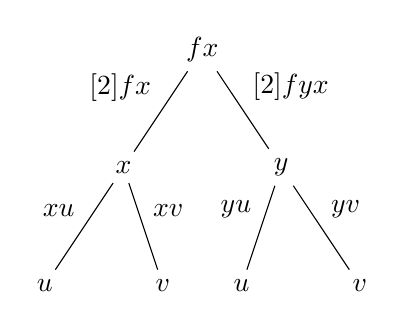
\begin{tikzpicture}
        \node (f) at (0,0) {$ \pdv{f}{x} $};  
        \node (x) at (-1,-1.5) {$x$};  
        \node (y) at (1,-1.5) {$y$};  
        \node (ux) at (-2,-3) {$u$};  
        \node (vx) at (-0.5,-3) {$v$};  
        \node (uy) at (0.5,-3) {$u$};  
        \node (vy) at (2,-3) {$v$};  
        \draw (f) edge node[midway,above left] {$ \pdv[2]{f}{x}$} (x) ;
        \draw (f) edge node[midway,above right] {$ \pdv[2]{f}{y}{x}$} (y) ;
        \draw (x) edge node[midway,above left] {$ \pdv{x}{u}$} (ux) ;
        \draw (x) edge node[midway,above right] {$ \pdv{x}{v}$} (vx) ;
        \draw (y) edge node[midway,above left] {$ \pdv{y}{u}$} (uy) ;
        \draw (y) edge node[midway,above right] {$ \pdv{y}{v}$} (vy) ;
      \end{tikzpicture}  
    \end{center}

    \begin{center}
      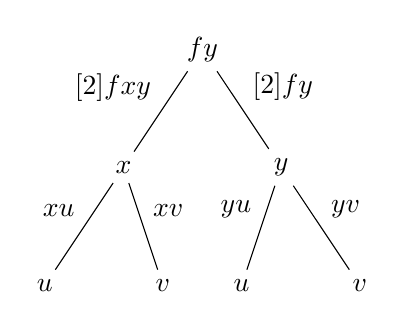
\begin{tikzpicture}
        \node (f) at (0,0) {$ \pdv{f}{y} $};  
        \node (x) at (-1,-1.5) {$x$};  
        \node (y) at (1,-1.5) {$y$};  
        \node (ux) at (-2,-3) {$u$};  
        \node (vx) at (-0.5,-3) {$v$};  
        \node (uy) at (0.5,-3) {$u$};  
        \node (vy) at (2,-3) {$v$};  
        \draw (f) edge node[midway,above left] {$ \pdv[2]{f}{x}{y}$} (x) ;
        \draw (f) edge node[midway,above right] {$ \pdv[2]{f}{y}$} (y) ;
        \draw (x) edge node[midway,above left] {$ \pdv{x}{u}$} (ux) ;
        \draw (x) edge node[midway,above right] {$ \pdv{x}{v}$} (vx) ;
        \draw (y) edge node[midway,above left] {$ \pdv{y}{u}$} (uy) ;
        \draw (y) edge node[midway,above right] {$ \pdv{y}{v}$} (vy) ;
      \end{tikzpicture}  
    \end{center}
  }{
    \begin{proof}
      \[
        \begin{aligned}
          \pdv[2]{f}{u} 
  &= \pdv{}{u}\left(\pdv{f}{u}\right) = \pdv{}{u} 
  \left( \pdv{f}{x} \pdv{x}{u} + \pdv{f}{y} \pdv{y}{u}\right) = 
  \pdv{}{u} \left(\pdv{f}{x} \pdv{x}{u}\right) + \pdv{}{u} 
  \left(\pdv{f}{y} \pdv{y}{u}\right) \\
  &= \pdv{}{u} \left( \pdv{f}{x}\right) \pdv{x}{u} + \pdv{f}{x} \pdv{}{u} \left(
  \pdv{x}{u} \right) + \pdv{}{u} \left(\pdv{f}{y} \right) \pdv{y}{u} + \pdv{f}{y} 
  \pdv{}{u} \left(\pdv{y}{u}\right) \\
  &=\left[ \pdv[2]{f}{x} \pdv{x}{u} + \pdv[2]{f}{x}{y} \pdv{y}{u} \right] \pdv{x}{u} +
  \pdv{f}{x} \pdv[2]{x}{u} + 
  \left[ \pdv[2]{f}{y}{x} \pdv{x}{u} + \pdv[2]{f}{y} \pdv{y}{u} \right] \pdv{y}{u} +
  \pdv{f}{y} \pdv[2]{y}{u} \\
  &= \pdv[2]{f}{x} \left(\pdv{x}{u}\right)^{2} + \pdv[2]{f}{x}{y} \pdv{y}{u}
  \pdv{x}{u} + \pdv{f}{x} \pdv[2]{x}{u} + \pdv[2]{f}{y}{x} \pdv{x}{u} \pdv{y}{u} + 
  \pdv[2]{f}{y} \left(\pdv{y}{u}\right)^{2} +
  \pdv{f}{y} \pdv[2]{y}{u} \\
  &= \pdv[2]{f}{x} \left(\pdv{x}{u}\right)^{2} + 2\pdv[2]{f}{x}{y} \pdv{x}{u}
  \pdv{y}{u} + \pdv[2]{f}{y} \left(\pdv{y}{u}\right)^{2} + \pdv{f}{x} \pdv[2]{x}{u} +
  \pdv{f}{y} \pdv[2]{y}{u} \\
        \end{aligned}
      \]
    \end{proof}
  }


  \subsection{Απόδειξη με το συμβολισμό των δεικτών}

  Αποδεικνύουμε τον τύπο για την $ f_{uu} $ και ομοίως προκύπτουν και οι τύποι για τις  
  $ f_{vv} $ και $ f_{uv} $.

  \vspace{\baselineskip}

  \twocolumnsideslc{
    \begin{center}
      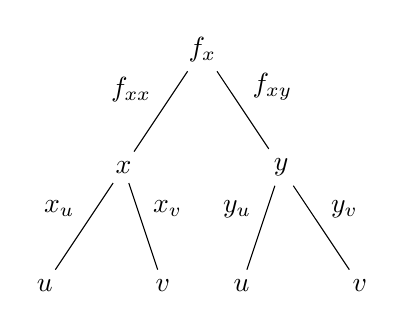
\begin{tikzpicture}
        \node (f) at (0,0) {$f_{x}$};  
        \node (x) at (-1,-1.5) {$x$};  
        \node (y) at (1,-1.5) {$y$};  
        \node (ux) at (-2,-3) {$u$};  
        \node (vx) at (-0.5,-3) {$v$};  
        \node (uy) at (0.5,-3) {$u$};  
        \node (vy) at (2,-3) {$v$};  
        \draw (f) edge node[midway,above left] {$f_{xx}$} (x) ;
        \draw (f) edge node[midway,above right] {$f_{xy}$} (y) ;
        \draw (x) edge node[midway,above left] {$x_{u}$} (ux) ;
        \draw (x) edge node[midway,above right] {$x_{v}$} (vx) ;
        \draw (y) edge node[midway,above left] {$y_{u}$} (uy) ;
        \draw (y) edge node[midway,above right] {$y_{v}$} (vy) ;
      \end{tikzpicture}
    \end{center}

    \begin{center}
      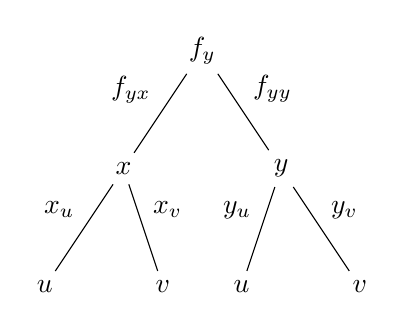
\begin{tikzpicture}
        \node (f) at (0,0) {$f_{y}$};  
        \node (x) at (-1,-1.5) {$x$};  
        \node (y) at (1,-1.5) {$y$};  
        \node (ux) at (-2,-3) {$u$};  
        \node (vx) at (-0.5,-3) {$v$};  
        \node (uy) at (0.5,-3) {$u$};  
        \node (vy) at (2,-3) {$v$};  
        \draw (f) edge node[midway,above left] {$f_{yx}$} (x) ;
        \draw (f) edge node[midway,above right] {$f_{yy}$} (y) ;
        \draw (x) edge node[midway,above left] {$x_{u}$} (ux) ;
        \draw (x) edge node[midway,above right] {$x_{v}$} (vx) ;
        \draw (y) edge node[midway,above left] {$y_{u}$} (uy) ;
        \draw (y) edge node[midway,above right] {$y_{v}$} (vy) ;
      \end{tikzpicture}
    \end{center}
  }{
    \begin{proof}
      \[
        \begin{aligned}
          f_{uu} &= (f_{u})_{u} = (f_{x}x_{u}+f_{y}y_{u})_{u} \\
                 &=(f_{x}x_{u})_{u}+ (f_{y}y_{u})_{u} \\
                 &=(f_{x})_{u}x_{u} + f_{x}(x_{u})_{u} + (f_{y})_{u}y_{u}+ 
                 f_{y}(y_{u})_{u} \\
                 &= (f_{xx}x_{u}+f_{xy}{y_{u}})x_{u} + f_{x} x_{uu} + 
                 (f_{yx}x_{u}+f_{yy}y_{u})y_{u} + f_{y}y_{uu} \\
                 &= f_{xx}(x_{u})^{2} + f_{xy}y_{u}x_{u}+ f_{x}x_{uu} + 
                 f_{yx}x_{u}y_{u}+f_{yy}(y_{u})^{2}+ f_{y}y_{uu} \\
                 &= f_{xx}(x_{u})^{2}+ 2f_{xy}x_{u}y_{u} + f_{yy}(y_{u})^{2} + 
                 f_{x}x_{uu} + f_{y}y_{uu}
        \end{aligned}
      \] 
    \end{proof}
  }

  \begin{rem}
    Συγκεντρωτικά οι τύποι για τις παραγώγους 2ης τάξης της συνάρτησης 
    \[
      f_{uu}= f_{xx}(x_{u})^{2}+ 2f_{xy}x_{u}y_{u} + f_{yy}(y_{u})^{2} + f_{x}x_{uu} + 
      f_{y}y_{uu} 
    \] 
    \[
      f_{vv}= f_{xx}(x_{v})^{2}+ 2f_{xy}x_{v}y_{v} + f_{yy}(y_{v})^{2} + f_{x}x_{vv} + 
      f_{y}y_{vv} 
    \]
    \[
      f_{uv}= f_{xx}x_{u}x_{v}+ f_{xy}(x_{u}y_{v} + x_{v}y_{u}) + 
      f_{yy}y_{u}y_{v} + f_{x}x_{uv} + f_{y}y_{v} 
      f_{y}y_{vv} 
    \]
  \end{rem}

  %todo συνθετη παραγωγος (φυσικο) να γράψω ασκήσεις με r, lnr κλπ

  \end{document}

